\documentclass[10pt,a4paper]{article}
\usepackage[T1]{fontenc}
\usepackage[utf8]{inputenc}
\usepackage{lmodern}
\usepackage[margin=25mm]{geometry}
\usepackage{amsmath,amssymb,booktabs,graphicx}
\usepackage{caption,float}
\usepackage[hidelinks]{hyperref}
\captionsetup{font=small}
\setlength{\parindent}{0pt}
\setlength{\parskip}{5pt}
\setlength{\emergencystretch}{2em}
\newcommand{\ind}{\mathbf{1}}
\newcommand{\Ptop}{\widehat{P}_{46}}
\begin{document}
\hypersetup{pdftitle={Point 3: Uncertainty in hazard ranks}}
\section*{Point 3: Uncertainty in hazard ranks}
\section{Evaluation setup}
We analyze hazard probabilities from $B=128$ separately fitted linear heads over
frozen DINOv3 ViT-B/16 features. Each head was trained on a bootstrap sample of
1,276 Pittsburgh training observations (527 hazards and 749 non-hazards), with
exact-pixel clusters sampled within strata defined by their binary-label composition.
All heads used Adam, learning rate $3\times10^{-5}$, weight decay $0.01$, batch
size 64, 5,000 updates, unweighted binary cross-entropy, and the final checkpoint.

The validation set contains 382 observations, including 157 hazards; the test set
contains 380 observations, including 174 hazards. The review budget is fixed at
$k=46$: 12.04\% of validation and 12.11\% of test. For an ordering $\pi$, the metrics are
\begin{equation}
\operatorname{Precision@46}=\frac{1}{46}\sum_{a=1}^{46}y_{\pi(a)},
\qquad
\operatorname{Recall@46}=\frac{\sum_{a=1}^{46}y_{\pi(a)}}{\sum_{i=1}^{N}y_i},
\end{equation}
where $y_i=1$ denotes a hazard. Subtype predictions are excluded.

\section{Rank distributions and pairwise probabilities}
For each head, rank all observations together by decreasing hazard probability,
with rank 1 the highest. Let $r_i^{(b)}$ be the resulting rank, using midranks for
exact probability ties. We summarize
\begin{equation}
\overline{r}_i=\frac{1}{B}\sum_{b=1}^{B}r_i^{(b)},\qquad
I_i=\left[Q_{0.025}(r_i^{(1:B)}),\ Q_{0.975}(r_i^{(1:B)})\right].
\end{equation}
Quantiles use linear interpolation. These are intervals of midranks across
refits; they do not include hypothetical random tie-breaking noise.

For selection frequencies, tied slots are allocated equally. If head $b$ assigns
$a_i^{(b)}$ observations strictly higher scores and $t_i^{(b)}$ observations the
same score (including $i$), define
\begin{equation}
\widehat{P}_{k}(i)=\frac{1}{B}\sum_{b=1}^{B}
\min\!\left\{1,\max\!\left\{0,\frac{k-a_i^{(b)}}{t_i^{(b)}}\right\}\right\}.
\end{equation}
We report $\widehat{P}_1(i)$ and $\widehat{P}_{46}(i)$. Their sums over images are
1 and 46, respectively. These frequencies quantify selection stability across
heads, not the probability that an image is a true hazard.

For each image pair, compare predictions from the same head:
\begin{equation}
W_{ij}=\frac{1}{B}\sum_{b=1}^{B}\ind\!\left[p_i^{(b)}>p_j^{(b)}\right],\qquad
T_{ij}=\frac{1}{B}\sum_{b=1}^{B}\ind\!\left[p_i^{(b)}=p_j^{(b)}\right].
\end{equation}
Then $W_{ij}+W_{ji}+T_{ij}=1$, $W_{ii}=0$ and $T_{ii}=1$. Matching head indices
preserves dependence between predictions. In particular,
\begin{equation}
\overline{r}_i=1+\sum_{j\ne i}\left(W_{ji}+\tfrac12 T_{ij}\right),
\end{equation}
so sorting by increasing expected rank is equivalent to weighted Borda ordering.
We compare this primary ordering with mean probability and decreasing
$\widehat{P}_{46}$. Ties in selection frequency are broken by expected rank, then
sample ID; equal expected ranks use sample ID. No labels determine these orderings.

\section{Retrieval results}
\begin{table}[H]
\centering
\caption{Hazard retrieval at the fixed budget of 46 images. Precision and recall are percentages.}
\label{tab:ranks}
\small
\begin{tabular}{llrrr}
\toprule
Split & Ranking & Hazards & Precision@46 & Recall@46 \\
\midrule
Validation & Mean probability & 34/46 & 73.91 & 21.66 \\
 & Expected rank & 34/46 & 73.91 & 21.66 \\
 & Top-46 frequency & 34/46 & 73.91 & 21.66 \\
\midrule
Test & Mean probability & 27/46 & 58.70 & 15.52 \\
 & Expected rank & 27/46 & 58.70 & 15.52 \\
 & Top-46 frequency & 28/46 & 60.87 & 16.09 \\
\bottomrule
\end{tabular}
\end{table}

All three methods retrieve 34 validation hazards (73.91\%). Mean and expected-rank
orderings retrieve 27 test hazards (58.70\%); top-46 frequency retrieves 28
(60.87\%). The frequency ordering replaces one selected test non-hazard with a
hazard, a 2.17 percentage-point difference. Neither the mean nor the frequency
ordering has a tie at its test selection boundary. The validation score does not
distinguish the methods, and the test difference is not used to select a winner.

\section{Rank stability}
\begin{table}[H]
\centering
\caption{Stability across 128 heads. Interval widths are measured in rank positions; other rows count observations.}
\label{tab:stability}
\small
\begin{tabular}{lrr}
\toprule
Statistic & Validation & Test \\
\midrule
Median rank-interval width & 156.2 & 162.2 \\
90th-percentile interval width & 208.4 & 215.8 \\
Intervals crossing rank 46 & 100 & 112 \\
Images with $\widehat{P}_{46}\geq0.95$ & 14 & 14 \\
Hazards among these stable selections & 9 & 8 \\
Non-hazards among these stable selections & 5 & 6 \\
Images with $\widehat{P}_{46}>0$ & 158 & 171 \\
\bottomrule
\end{tabular}
\end{table}

The test median rank-interval width is 162.2 positions, and 112 intervals cross
the review cutoff. Only 14 test images appear in the top 46 in at least 95\% of
heads. Of these, 8 are labelled hazards and 6 non-hazards. Thus, stability can
coexist with systematic false-positive selections. Mean and expected-rank
orderings nevertheless select exactly the same 46 images on each split: agreement
between their aggregate selections does not imply narrow per-image rank intervals.

\section{Interpretation and limitations}
Rank intervals show where placement is sensitive to refitting, while top-46
frequency identifies stable review candidates. These quantities can accompany a
ranking without changing its ordering. The one-image test gain from frequency
ranking is descriptive and does not establish general superiority or statistical
significance. The pairwise probabilities also quantify whether any particular
comparison is well supported by the ensemble, rather than forcing every ordering
to appear equally certain.

The 128 heads share a frozen representation and overlapping bootstrap training
samples. Their variation measures sensitivity to these model refits, not all
sources of predictive uncertainty. Empirical intervals are not automatically
calibrated posterior intervals or confidence intervals for population precision.
Original evaluation observations are retained, including duplicate pixel groups
and groups with conflicting hazard labels: 18 duplicate groups, of which 6 have
conflicting labels, in validation; 12 and 2, respectively, in test. Shared confident
mistakes and label conflicts can therefore persist across the ensemble.

\clearpage
\section{Rank-uncertainty figures}
\begin{figure}[H]
\centering
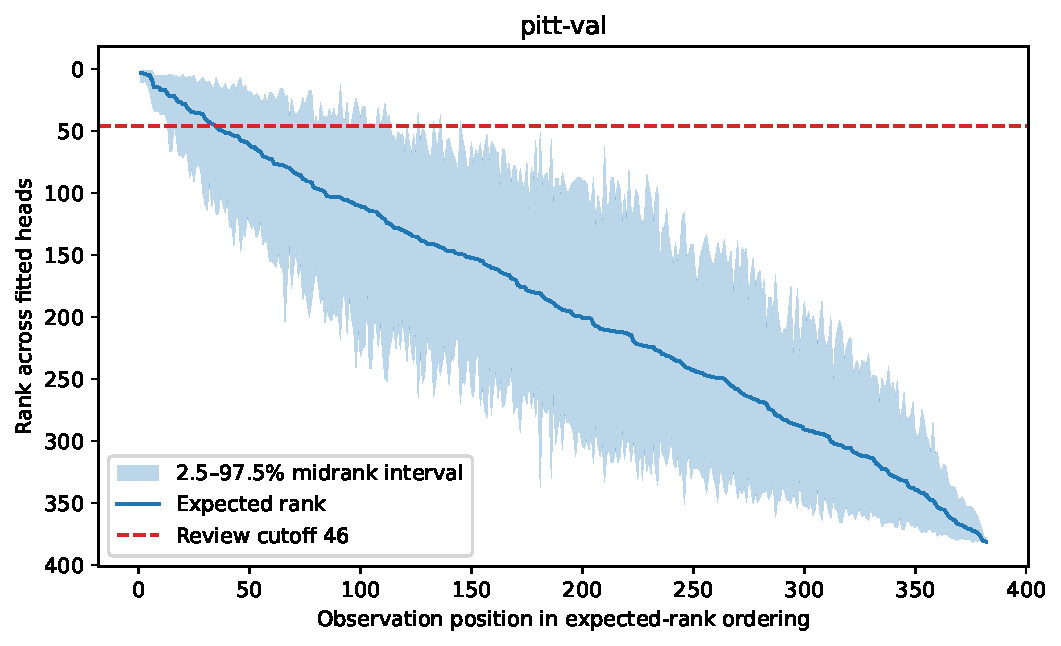
\includegraphics[width=.9\linewidth]{figures/point_3_pitt-val_rank_intervals.pdf}
\caption{Validation rank intervals. Observations are ordered by expected rank; shading shows the 2.5th--97.5th percentile interval and the dashed line marks rank 46.}
\label{fig:val-rank}
\end{figure}
\begin{figure}[H]
\centering
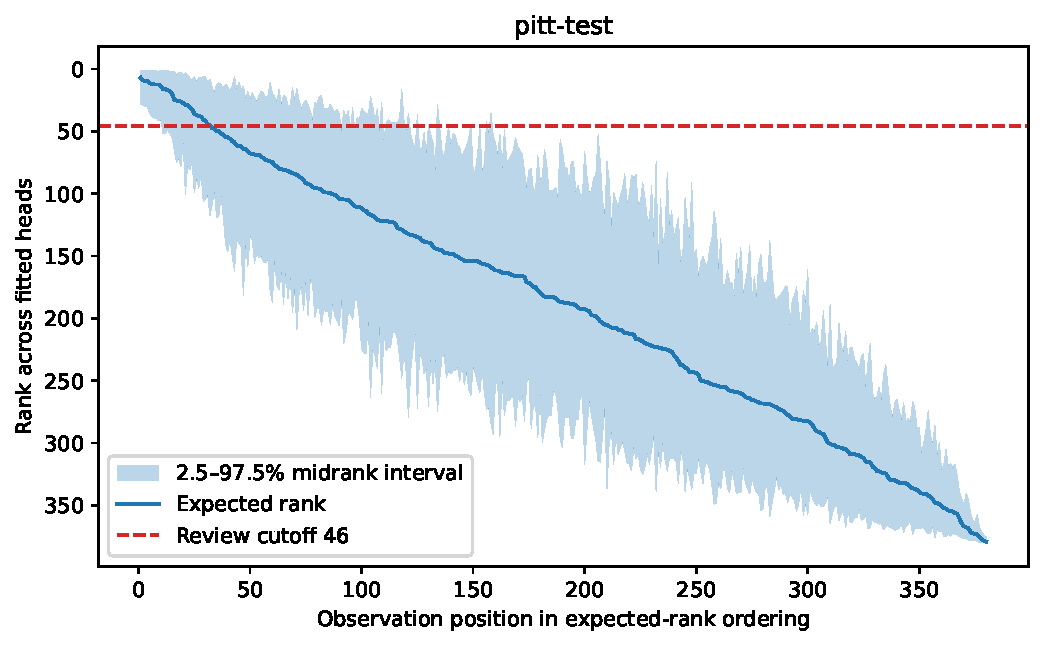
\includegraphics[width=.9\linewidth]{figures/point_3_pitt-test_rank_intervals.pdf}
\caption{Test rank intervals, with the same definition. Smaller ranks are better, so the vertical axis increases downwards.}
\label{fig:test-rank}
\end{figure}
\begin{figure}[H]
\centering
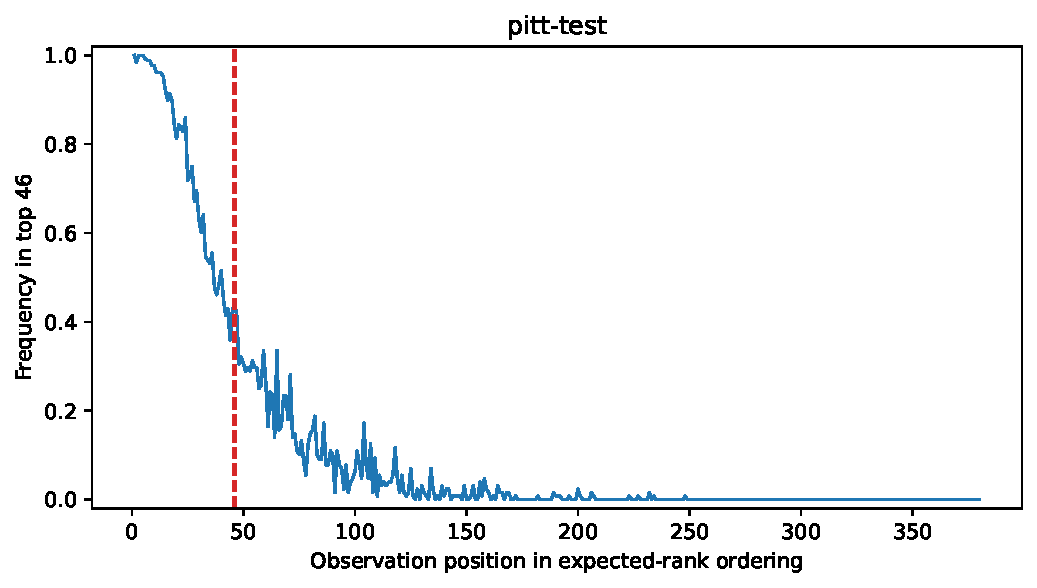
\includegraphics[width=.9\linewidth]{figures/point_3_pitt-test_top_k_frequency.pdf}
\caption{Test top-46 selection frequencies, plotted in expected-rank order. The vertical line marks the first 46 positions of that aggregate ordering.}
\label{fig:test-frequency}
\end{figure}

\end{document}
